\documentclass{article}\usepackage[margin=1in]{geometry}\usepackage{booktabs}\usepackage{graphicx}\usepackage{xcolor}\usepackage{hyperref}
\title{Love AI More. Trust AI Less.}\author{DSCT lecture walkthrough}\date{}
\begin{document}\maketitle
\begin{abstract}A short report can be a reasoning instrument: state a claim, inspect evidence, and decide how much confidence is earned.\end{abstract}
\section{The question}\textbf{Claim:} Increasing simultaneous requests should increase aggregate AI throughput until parallelism is saturated. This matters because “bigger GPU is faster” can confuse capacity with scheduling.
\section{Evidence}\begin{tabular}{llrrrr}\toprule
Hardware & parallel limit & $N=1$ & $N=4$ & $N=8$ & $N=32$\\\midrule
Tesla T4 & 1 & 69.2 / 0.49 & 74.1 / 0.54 & 73.4 / 0.53 & 73.4 / 0.54\\
Tesla T4 & 8 & 72.6 / 0.53 & 102.8 / 2.18 & 117.3 / 4.77 & 121.9 / 4.84\\
GTX 1060 3 GB & 1 & 59.6 / 0.61 & 84.5 / 0.86 & 90.2 / 0.92 & 94.6 / 0.98\\
GTX 1060 3 GB & 4 & 73.6 / 0.99 & 112.1 / 3.76 & 120.7 / 3.98 & 119.9 / 3.97\\
\bottomrule
\multicolumn{6}{l}{\scriptsize Each cell: aggregate tokens/s \,/\, overlap factor.}\\
\end{tabular}
\begin{figure}[h]\centering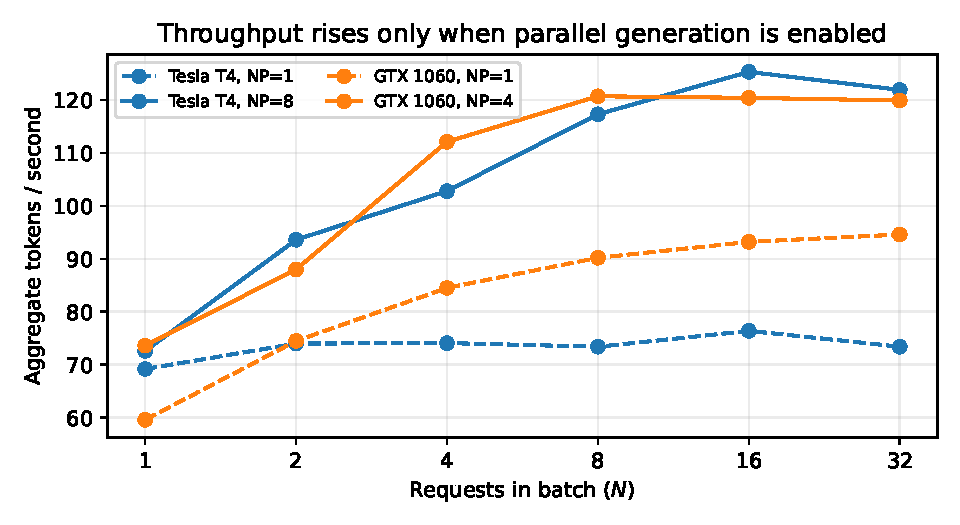
\includegraphics[width=.9\linewidth]{../../generated/figures/throughput.pdf}\caption{Aggregate throughput across six batch sizes.}\end{figure}
\end{document}
